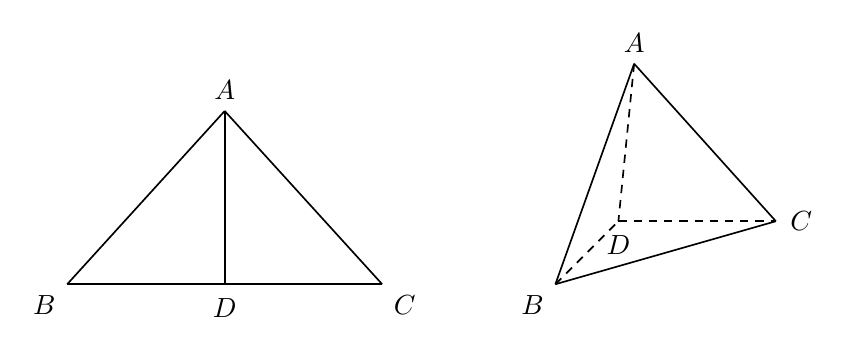
\begin{tikzpicture}[x=1cm,y=1cm,font=\normalsize]
\tikzset{edge/.style={draw=black,line width=.6pt,solid},hedge/.style={draw=black,line width=.6pt,dashed,dash pattern=on 3pt off 2.5pt},lbl/.style={font=\normalsize,inner sep=2pt}}
\coordinate (LA) at (2.0,2.2);
\coordinate (LB) at (0,0);
\coordinate (LC) at (4.0,0);
\coordinate (LD) at (2.0,0);
\coordinate (RA) at (7.2,2.8);
\coordinate (RB) at (6.2,0);
\coordinate (RC) at (9.0,0.8);
\coordinate (RD) at (7.0,0.8);
\draw[edge] (LA) -- (LB);
\draw[edge] (LA) -- (LC);
\draw[edge] (LB) -- (LC);
\draw[edge] (LA) -- (LD);
\draw[edge] (RA) -- (RB);
\draw[edge] (RA) -- (RC);
\draw[edge] (RB) -- (RC);
\draw[hedge] (RA) -- (RD);
\draw[hedge] (RB) -- (RD);
\draw[hedge] (RD) -- (RC);
\node[lbl,above,yshift=2pt] at (LA) {$A$};
\node[lbl,below left,xshift=-2pt,yshift=-2pt] at (LB) {$B$};
\node[lbl,below right,xshift=2pt,yshift=-2pt] at (LC) {$C$};
\node[lbl,below,yshift=-3pt] at (LD) {$D$};
\node[lbl,above,yshift=2pt] at (RA) {$A$};
\node[lbl,below left,xshift=-2pt,yshift=-2pt] at (RB) {$B$};
\node[lbl,right,xshift=3pt] at (RC) {$C$};
\node[lbl,below,yshift=-3pt] at (RD) {$D$};
\end{tikzpicture}
